% !TEX encoding = UTF-8 Unicode

% **CONSIGNES
%	- 12 pages maximum (annexes incluses)
%	- Sans changer la mise en page du template.

% **STRUCTURE
%	1. l’INTRODUCTION présente la problématique (projet) ;
%	2. la PARTIE PRINCIPALE, articulée suivant la problématique d’étude:
%		- présente les données et les analyses effectuées, de manière structurée;
%	3. la CONCLUSION:
%		- résume les résultats
%		- présente d’éventuelles perspectives d’études dont la mise en oeuvre dépasse le cadre du TP;
%	4. d’éventuelles annexes contiennent:
%		- le code,
%		- les figures si elles sont trop nombreuses pour être mises dans le texte,
%		- les détails de calculs un peu longs.

% **MISE EN PAGE
% *italique*:
%		-On évitera de mettre un élément d’information en valeur au moyen de caractères gras ou d’une police soulignée, on préfère en général utiliser l’italique pour cela.
% *tableau et figures*:
%		- On évitera d’afficher trop de tableaux ou de figures. Ceux qui seront choisis devront être optimisés, de manière à communiquer autant d’informations pertinentes que possible en un minimum de place. Évitez les tableaux ou figures orphelins (sans légende, pas numérotés, sans référence, laissés à eux-mêmes dans le corps du texte) ! Notons que par convention, la légende se met en haut pour un tableau et en bas pour une figure.
% 		- Les couleurs et les symboles permettent d’ajouter une information supplémentaire parfois précieuse (voir par exemple la figure 1, où la couleur représente l’espèce d’iris). Toutefois, les documents étant presque exclusivement imprimés en noir et blanc, on préférera en général l’utilisation de symboles spécifiques.
% *code source*: 
%		- devrait être évité dans le compte-rendu, à moins qu’ils ne présente un intérêt particulier ou ne soit absolument nécessaire à la compréhension (ce qui n’est généralement pas le cas). La mention d’un petit nombre de commandes est tolérable, si c’est nécessaire.
% *analyse*: 
%		- dépasser les commentaires triviaux (tels que « la méthode marche mal », ou encore « la méthode donne tel résultat »), qui trahissent un manque de réflexion et sont donc généralement sanctionnés.
% *cohérence*: 
%		- vos différentes contributions devront être articulées. Vous insisterez sur les aspects complémentaires des traitements que vous aurez mené (comme par exemple lorsqu’un test statistique vient compléter une représentation graphique).


%\documentclass[twoside]{article}
\documentclass[twocolumn,10pt]{article}
\usepackage[french]{babel}
\usepackage[utf8]{inputenc}
\usepackage[T1]{fontenc}

\usepackage{amsmath}
\usepackage{amssymb}
\usepackage{amsfonts}
\usepackage{graphicx}
\usepackage{bbm}

\usepackage[margin=2cm,top=32mm,columnsep=20pt]{geometry}
\usepackage{multirow,multicol} % Style double colonne 
\usepackage{abstract} % Customization de l'abstract 
\usepackage{fancyhdr} % en-têtes et pieds de page 
\usepackage{float} % Nécessaire pour les tables et figures dans l'environnement double colonne 

\usepackage{enumitem,xcolor}
\usepackage[french]{algorithm2e}%linesnumbered

\usepackage[colorlinks=true,linkcolor=red,urlcolor=blue,filecolor=green]{hyperref} % hyperliens 
\usepackage{dtk-logos}


%----------------------------------------------------------------------------------------
\setlength{\parskip}{1ex} % espace entre paragraphes 

% Affichage du code python 
\usepackage[cachedir=cache/minted-\jobname]{minted}
\setminted{encoding=utf8, numbersep=3pt, xleftmargin={2em}, breaklines, linenos=true}
\def\Rcode#1{\mintinline{R}{#1}}
\def\pycode#1{\mintinline{python}{#1}}


%----------------------------------------------------------------------------------------
% En-têtes et pieds de page 
\pagestyle{fancy}  
% En-tête de page
\fancyhead{} % Blank out the default header
\fancyhead[L]{SY09}
\fancyhead[C]{\textit{Russian troll tweets}}
\fancyhead[R]{D4\_G6}
% Pied de page
\fancyfoot{} % Blank out the default footer
\fancyfoot[RO,LE]{\thepage}

\title{\textsc{Compte-rendu d'analyse}}
\author{François \textsc{Marès}\\ Merwan \textsc{Bouvier}\\ Thomas \textsc{Laurent}}
\date{\today}


\begin{document}

\maketitle % Insert title
\thispagestyle{fancy} % All pages have headers and footers

\begin{abstract}
Les près de 3 millions de tweets associés à l'\textit{Internet Research Agency}, une organisation impliquée dans la campagne d'influence russe des élections américaines de 2016, peuvent faire l'objet d'une classification comportementale. Les chercheurs Darren Linvill et Patrick Warren ont proposé une telle classification, comprenant essentiellement les classes \textit{Right Troll}, \textit{Left Troll}, \textit{News Feed} et \textit{Hashtag Gamer}. Nous discutons dans ce document de plusieurs méthodes candidates pour automatiser cette classification avec le plus de précision possible. 

Après avoir défini une stratégie de représentation du contenu sémantique des tweets, nous éprouvons plusieurs méthodes pour parvenir à mettre en avant celle capable de distinguer le mieux possibles les comportements principaux des comptes trolls.


\end{abstract}


%----------------------------------------------------------------------------------------

\section{Introduction}\label{sec:introduction}

En janvier 2017, la CIA, le FBI et la NSA publient un document conjoint dont la version déclassifiée\cite{ODNI17} contient des jugements relatifs aux activités russes en rapport avec les élections présidentielles américaines de 2016. Il affirme qu'une politique d'influence de la démocratie américaine favorable à Trump a été mise en œuvre, et énonce les moyens employés. En particulier, est écrit que la stratégie russe \textit{allie des opérations secrètes de renseignement aux efforts manifestes des agences gouvernementales russes, des médias financés par l'État, des intermédiaires tiers et des utilisateurs rémunérés des médias sociaux ou «trolls»}.

En février, l'\textit{Internet Research Agency} (IRA), organisation basée à Saint-Pétersbourg identifiée comme la source des trolls russes, est mise en examen pour ses activités. Le rapport du procureur spécial\cite{SCRM19}, publié en 2019, conclut à l'absence de collusion entre la Russie et Trump, mais présente de nombreux éléments sur les opérations russes -- cependant presque tous les détails, en particulier ceux sur les tweets de l'IRA (p.24), sont noircis.

En juillet 2018, le site web \textit{FiveThirtyEight}, spécialisé dans le journalisme de données, donne accès librement à des fichiers contenant près de 3 millions de tweets associés à l'IRA \cite{OR18}. Cette base de données a été constituée par deux chercheurs de l'Université de Clemson, Darren Linvill et Patrick Warren, à partir des informations que Twitter a fourni au Congrès américain sur les comptes trolls et leurs agissements entre mai 2015 et novembre 2017. Les chercheurs s'en sont servis pour étudier les méthodes d'influence de la politique américaine par l'IRA \cite{DLPW18}. Pour ce faire, il ont classifié les activités des comptes en thèmes, par exemple \textit{Left Troll} ou \textit{Right Troll}.

L'objectif de notre étude est d'automatiser cette classification des tweets en provenance de l'\textit{usine à trolls} russe, grâce à des méthodes d'apprentissage supervisé.

Faciliter l'étude des campagnes de désinformations est nécessaire pour qui souhaiterait prendre des mesures capables de limiter leur efficacité. Cet objectif fait parti de ceux de Twitter: depuis la révélation de l'affaire des trolls russes, l'entreprise a annoncé la suppression de nombreux comptes liés à des opérations d'influence.

%------------------------------------------------

\section{Analyse}\label{sec:contenu}

%Après une présentation des données, cette partie rend compte de la démarche de notre analyse ainsi que des résultats obtenus.

\subsection{Présentation des données}

La base de données contient près de 3 000 000 de tweets provenant de seulement 2 848 pseudonymes Twitter. Ils ont été envoyés entre février 2012 et mai 2018 mais la grande majorité a été postée de 2015 à 2017. L'activité des comptes est fortement corrélée avec les évènements médiatiques majeurs liés à la politique aux États-Unis -- la vérification du contenu des tweets vient confirmer ce lien. C'est particulièrement remarquable pour l'année 2016 [\textsc{Figure}~\ref{fig:C2016}], année d'élection de Donald Trump à la Maison Blanche.

\begin{figure}[h]
\begin{center}
\caption{\label{fig:C2016}Chronologie des tweets publiés en 2016.}
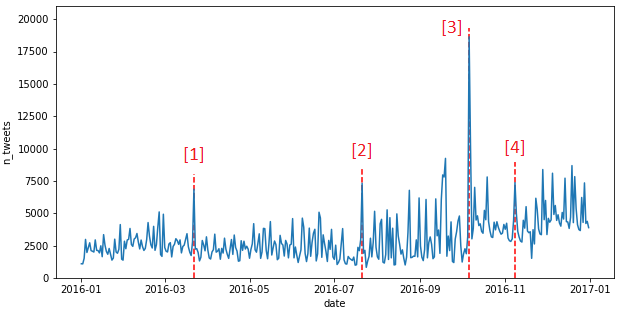
\includegraphics[width=0.45\textwidth]{Ressources/2016_tweets.png}
\end{center}
\end{figure}

\begin{enumerate}[label={\color{red}[\theenumi]}]
\item Mars 2016, WikiLeaks publie plus de 30 000 courriels et pièces jointes de la messagerie privé d'Hillary Clinton alors qu'elle était secrétaire d'État.
\item Juillet 2016, Investiture de Donald Trump comme candidat républicain.
\item Octobre 2016, fuite de milliers de nouveaux mails d'Hillary Clinton.
\item 8 novembre 2016, Donald Trump est élu quarante-cinquième président des États-Unis. 
\end{enumerate}

\subsubsection{Catégories de Linvill et Warren}

Les tweets et comptes associés ont été classés en 8 groupes comportementales par Linvill et Warren, dont voici une brève description (par ordre décroissant de tweets associés):
\begin{description}
\item[Non English (837,725)] Comptes rédigeant le plus souvent dans une autre langue que l'anglais -- le plus fréquemment il s'agit du russe.

\item[Right Troll (719,087)] Comptes se faisant passer pour des supporters de Donald Trump. Ils publient des tweets aux messages populistes républicains, dénigrent Obama et Hillary Clinton.
\item[News Feed (599,294)]  Comptes se faisant passer pour des agrégateurs de nouvelles locales officielles partageant les actualités autour de certaines villes américaines.
\item[Left Troll (427,811)] En opposition aux \textit{Right Trolls}, cette catégorie se fait passer pour des activistes supporters du parti Démocrate. Ils ont pour but de diviser le parti Démocrate et critiquent pour certains Hillary Clinton.
\item[Hashtag Gamer (241,827)] Comptes publiant selon le jeux hashtag -- l'utilisateur met un hashtag spécifique et répond à la question impliqué par celui-ci. Le but de cette catégorie est de se faire passer pour des joueurs de jeux vidéo et publier des tweets politiques de temps à autre, notamment à travers les jeux hashtag.
\item[Commercial (122,582)] Comptes à buts commerciaux. Leurs tweets décrivent un produit (perte de poids, investissement, etc.) souvent accompagné d'un lien et de mentions vers d'autres comptes twitter.
\item[Unknown (13,905)] Comptes inclassables parmi les autres catégories.
\item[Fearmonger (11,140)] Comptes propageant des informations sur des événements de crise inventés.
\end{description}

Bien que la catégorie \verb!Non English! soit importante dans les données, pour des raisons de difficultés de traduction nous ignorons cette catégorie dans notre analyse. La catégorie \verb!Unknown!, peu importante en volume sera elle aussi ignorée. Parmi les cinq modèles de comportement -- \textit{Right Troll}, \textit{Left Troll}, \textit{News Feed}, \textit{Hashtag Gamer} et \textit{Fearmonger} --,  \textit{Fearmonger} fait exception: les tweets des comptes de cette catégorie passent parfois d'une catégorie à une autre. C'est pourquoi nous avons choisi de ne pas en tenir compte pour la suite de notre analyse.

Nous restreignons donc notre problématique à l'automatisation de la classification des tweets en provenance de l'\textit{usine à trolls} russe parmi les quatre catégories \textit{Right Troll}, \textit{Left Troll}, \textit{News Feed} et \textit{Hashtag Gamer}.

\subsubsection{Restriction des données d'origine}

En plus de ne nous intéresser qu'à quatre catégories, nous retirons de notre analyse tous les tweets rédigés dans une autre langue que l'anglais. Notre étude porte finalement sur les deux-tiers des tweets de la base de données d'origine (1 959 778 tweets); par la suite, chaque fois que nous parlerons de données nous feront référence à ce sous-ensemble.

\subsubsection{Données d'entraînement et de test}

Pour que la comparaison entre les méthodes de classification automatique soit équitable, nous utiliserons toujours les mêmes données d'entraînement et de test. Nous avons séparé aléatoirement nos données en deux jeux: 80\% (soit 1 567 823 tweets) pour les données d'entraînement et les 20\% restantes (soit 391 955 tweets) pour les données de test.

Sauf précisions contraires, les statistiques évoquées par la suite porterons sur les seules données d'entraînement.

\subsubsection{Descripteurs candidats pour la classification}

Le jeu de données initial comporte 21 descripteurs pour chaque tweet:
\begin{multicols}{3}
\noindent external\_author\_id \\ %
author \\ %
content \\ 
region \\ %
language \\ %
publish\_date \\ %
harvested\_date \\ %
following \\ %
followers \\ %
updates \\ %
post\_type \\ %
account\_type \\ %
retweet \\ %
account\_category \\ %
new\_june\_2018 \\ %
alt\_external\_id \\ %
tweet\_id \\ %
article\_url \\ %
tco1\_step1 \\ %
tco2\_step1 \\ %
tco3\_step1 %
\end{multicols}

Cependant, la plupart ne sont pas pertinents pour notre classification.

Puisque, par ses tweets, c'est en réalité un compte que nous voulons classifier, tous les descripteurs qui permettent de l'identifier avec certitude sont à exclure (\textit{external\_author\_id}, \textit{author}, \textit{alt\_external\_id}). Nous aurions pu garder le nom des comptes, pour exploiter le lien sémantique qui existe parfois avec le thème principal de ce dernier -- en particulier pour les comptes \textit{NewsFeed} --, mais nous n'avons pas voulu entrer dans une telle analyse.

Le descripteur \textit{region} est presque identique pour tous les tweets (États-Unis) puisque nous avons sélectionné les tweets en anglais.

La date de publication (\textit{publish\_date}) n'est pas retenue puisque nous désirons que notre classifieur ne se limite pas à la période des tweets d'apprentissage.

Les métadonnées techniques telles que la date de collecte du tweet, un booléen indiquant si le tweet  vient de l'extension de la base de données fournie au Congrès, l'identifiant du tweet ou encore le lien vers celui-ci (respectivement \textit{harvested\_date}, \textit{new\_june\_2018}, \textit{tweet\_id} et \textit{article\_url}) ne sont pas retenus pour notre classifieur.

Les trois liens présents dans un tweet (\textit{tco1/2/3\_step1}) ne sont pas non plus directement retenus; étant donnée, d'une part, la difficulté d'analyse des liens inconnus des données d'entrainement, et d'autre part la faible probabilité qu'un ancien lien soit utilisé par un autre tweet ultérieurement. Si notre objectif avait été de nous limiter à la classification de tweets sur une courte période, ou si nous voulions prendre en compte le maximum d'informations, nous pourrions ajouter par exemple quatre nouvelles variables. Chacune serait le score des liens du tweet relatif à chaque catégorie (comme nous l'avons fait pour l'analyse sémantique des tweets, cf. \ref{sec:NDQ}), défini par exemple comme la somme des fréquences d'utilisations des trois liens -- où des sites référencés -- parmi les données d'apprentissages de la catégorie.

Cependant, on observe que le nombre de liens est un bon discriminant pour les classes \textit{Hashtag Gamers} et \textit{News Feed}. Les \textit{Hashtag Gamers} publient des tweets avec une fréquence de présence de lien beaucoup plus faible (0.26), tandis que les tweets avec 3 liens proviennent plus largement des comptes \textit{News Feed}. Une variable contenant le nombre de liens peut être utilisée par notre classifieur lorsqu'il inclura des variables qualitatives.

Le type du tweet (décrit par \textit{post\_type} et \textit{retweet}) pourrait être retenu pour notre classification automatique, en particulier lorsque nous utiliseront des arbres de décision. Jusque là, cette variable qualitative n'est pas prise en compte.

Mis à part le contenu du tweet, les trois variables restantes \textit{following}, \textit{followers} et \textit{updates} sont quantitatives. Elles pourraient facilement être utilisées comme entrées de notre classifieur, mais nous nous heurterions alors à un biais important. En effet les données qui sont à notre disposition ne proviennent que d'environ 3000 comptes différents. Si un tweet de l'ensemble de test proviennent d'un compte représenté dans les données d'entraînement il est très probable que le classifieur fasse ce lien: ces variables prendraient le rôle d'identifiants du compte. On peut illustrer ce problème en mettant en œuvre la méthode des k plus proches voisins: pour $k=3$ par exemple on obtient une précision de 98\% si le partage des tweets en données d'apprentissage et de test est indifférent aux comptes. Un moyen d'éviter ce problème serait de rendre qualitatives ces variables.

Finalement, c'est à partir du contenu des tweets que nous avons choisi de les classifiers dans un premier temps, les autres descripteurs candidats étant qualitatifs [\textsc{Table} \ref{tab:DCC}]. La partie suivante (Sec. \ref{sec:NDQ}) présente la transformation de ce descripteur très complexe en huit descripteurs quantitatifs -- que nous appellerons \textit{scores}.

\noindent\begin{table}[htbp]
\begin{center}
\begin{tabular}{cc|c}
descripteur d'origine & descripteurs dérivées & type \\
\hline 
content & 8 scores & quantitatif \\ 
tco1/2/3\_step1 & nombre de liens & qualitatif \\ 
post\_type & & qualitatif
\end{tabular} 
\caption{\label{tab:DCC}Descripteurs candidats pour la classification.}
\end{center} 
\end{table}


\subsubsection{Nouveaux descripteurs quantitatifs}\label{sec:NDQ}

Naturellement, un humain qui voit un tweet dont il ne connait pas l'origine juge du thème de celui-ci à partir de son contenu textuel. Souvent, l'identification de quelques mots clef suffit. Les hashtags, en particulier, sont utilisés a escient pour maximiser l'efficacité de cette analyse; le temps qui y est consacré par le lecteur étant presque instantané.

Nous voulons donc construire des descripteurs qui quantifient l'orientation des mots clef d'un teweet, soit une crédence en son appartenance à chaque classe selon ses mots et hashtags utilisés, en traitant à part les hashtags.

Pour chaque catégorie, nous avons construit une liste des 100 mots les plus fréquemment employés parmi les tweets de l'ensemble d'entraînement, qui ne font pas partie des mots les plus communs de la langue anglaise. L'occurrence de chaque mot est ensuite remplacée par la proportion qu'elle représente par rapport au nombre total d'occurrences dans la liste. La \textsc{table} \ref{tab:RTLTw} donne pour deux classes les dix premiers mots de ces classements.

\begin{table}[htbp]
\begin{center}
\noindent\begin{tabular}{r|cl|cl}
& \multicolumn{2}{c|}{\verb!RightTroll!} & \multicolumn{2}{|c}{\verb!LeftTroll!} \\ 
\hline 
1 & trump & 0.1025 & black & 0.0523\\
2 & obama & 0.0340 & trump & 0.0466\\
3 & just & 0.0324 & just & 0.0317\\
4 & hillary & 0.0279 & white & 0.0260\\
5 & breaking & 0.0276 & police & 0.0213 \\
6 & video & 0.0218 & love & 0.0195\\
7 & president & 0.0197 & after & 0.0163\\
8 & clinton & 0.0179 & need & 0.0161\\
9 & realdonaldtrump & 0.0168 & today & 0.0153\\
10 & america & 0.0165 & women & 0.0142\\
\end{tabular}
\caption{\label{tab:RTLTw} 10 mots les plus employés par les classes \textit{Right Troll} et \textit{Left Troll}.}
\end{center} 
\end{table}

Le score de chaque tweet selon une classe donnée est ensuite déterminé comme la somme des proportions de l'intersection entre les mots qu'il contient et les 100 mots les plus employés par cette catégorie. L'opération est identique pour les hashtags.

La distribution des scores est très similaire entre ceux d'un même type sur des classes différentes, mais la distribution est très différente entre les scores sur les mots ou sur les hashtags. La \textsc{table} \ref{tab:SBRT} donne la moyenne, l'écart-type, les quartiles et le maximum des scores des tweets pour la classe \textit{Right Troll}.

\begin{table}[htbp]
\begin{center}
\noindent\begin{tabular}{r|ll}
 & Mots & Hashtags \\ 
\hline 
count & 1 567 823 & 1 567 823\\
\vspace{1mm}
mean & 0.0184 & 0.0027 \\
std & 0.0344 & 0.0078 \\
min & 0 & 0 \\
25\% & 0 & 0 \\
50\% & 0.0064 & 0 \\
75\% & 0.0179 & 0 \\
max & 1.7439 & 0.2978 \\
\end{tabular}
\caption{\label{tab:SBRT} Statistiques basiques sur les scores pour la classe \textit{Right Troll}.}
\end{center} 
\end{table}

On remarque que les scores sur les hashtags sont très faibles et souvent nuls, comme le confirme la \textsc{table} \ref{tab:PTSN}, qui donne le pourcentage de tweets avec un score nul pour chacun des huit descripteurs. Une raison commune à la faiblesse des scores sur les hashtags ainsi que de telles proportions de scores nuls est le peu de hashtags contenus dans chaque tweet, et le choix de ne prendre en compte que les 100 hashtags les plus fréquemment utilisés par les catégories. Pour le cas des hashtags des tweets de catégorie \textit{Hashtag Gamer}, les tweets utilisent des hashtags très variés, d'où les scores observés. Ce descripteur ne servira à discriminer la classe que de seulement quelques tweets -- en cas de besoin de réduire la dimension des données d'entrée de modèles, nous pourrons ignorer ce score.


\begin{table}[htbp]
\begin{center}
\noindent\begin{tabular}{r|ll}
 & Mots (\%) & Hashtags (\%)\\ 
\hline 
RightTroll & 43 & 83 \\
LeftTroll & 43 & 86 \\
NewsFeed & 52 & 84 \\
HashtagGamer & 50 & 99 \\
\end{tabular}
\caption{\label{tab:PTSN} Pourcentage des tweets au score nul pour chaque type de score.}
\end{center} 
\end{table}

\subsubsection{Limite des scores définis}\label{sec:limitescores}

Plus embêtant, 323 588 tweets (soit 20\% des données) ont tous leurs scores nuls, parce qu'ils s'éloignent des tweets typiques de leurs catégories -- ou même ne contiennent aucune information sémantique trahissant leur appartenance à un groupe comportemental.

Ces dernières remarques nous font anticiper que nos classifieurs sur les tweets n'auront surement pas une grande précision: une partie des tweets ne sont pas caractéristiques d'une catégorie comportementale, et nos scores ne rendent pas compte de toute l'information sémantique contenue dans un tweet.

Un moyen de pallier ce problème est, comme nous le faisons à la fin de l'analyse, de préférer comme mesure de précision celle concernant la prédiction de la catégorie des comptes (par le vote des prédictions sur ses tweets) plutôt que de celle des tweets isolés.


\subsubsection{Corrélations des scores}

Le coefficient de Spearman permet de décrire à quel point la dépendance entre deux variables est monotone\footnote{Nous aurions aussi pu choisir le coefficient des rangs de Kendall, moins sensible aux nombreuses valeurs nulles de nos scores, mais les résultats sont très proches.}. Plus une telle relation entre les variables est marquée, plus le coefficient se rapproche de 1 en valeur absolue.

Les coefficient de Spearman des huit variables score sont représentés sur la \textsc{figure} \ref{fig:MCS}.

\begin{figure}[h]
\begin{center}
\caption{\label{fig:MCS}Matrice de corrélations de Spearman (valeurs absolues).}
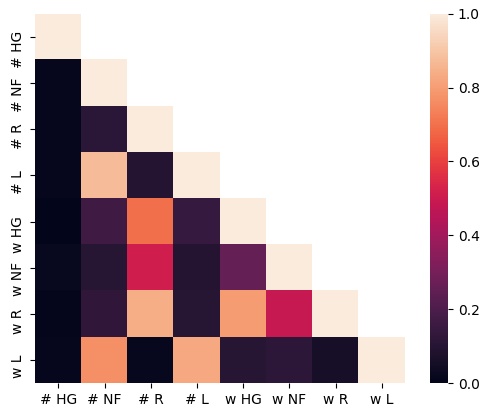
\includegraphics[width=0.45\textwidth]{Ressources/matrice_correlations.png}
\end{center}
\end{figure}

Pour nos descripteurs, la monotonie des dépendances n'est pas un indicateur suffisant pour juger de leur capacité de discrimination, mais une forte monotonie de dépendances est mauvais signe. En effet, si deux scores évoluent l'un par rapport à l'autre toujours de la même manière -- par exemple sont proportionnelles si le coefficient de Pearson est proche de 1 en valeur absolue --, alors il y a un risque que les deux variables soient de mauvais discriminants entre les deux catégories associées. Les scores associés aux classes \textit{News Feed} et surtout \textit{Hashtag Gamers} sont les plus monotonement corrélées aux autres classes, on peut s'attendre à des difficultés de classifications les concernant.

À l'opposé, il est bon que le coefficient de corrélation entre le score sur les mots et sur les hashtags pour une même catégorie soit élevé. C'est le cas pour les classes \textit{Left Troll} et \textit{Right Troll}.



\subsection{Apprentissages supervisés}

\subsubsection{Classifications triviales à battre}

Commençons par évoquer les méthodes de classifications triviales qui serviront de référence pour interpréter les résultats des méthodes plus avancées.

Sans apprentissage, la probabilité à priori qu'un tweet appartienne à une parmi quatre classes est de 0.25. Un classifieur naïf pourrait tirer au hasard la classe de chaque tweet [\textit{N.1}].

Ou bien, comme la répartition parmi les classes n'est pas égale dans les données, tirer au hasard selon les probabilités à postériori d'appartenir à une classe, selon les proportions des données d'entraînement [\textit{N.2}].

Enfin, une troisième méthode simple est de prendre pour prédiction la catégorie associée au meilleur score parmi les huit définis [\textit{S.0}], ou seulement les scores sur les mots [\textit{Sw.0}], ou sur les hashtags [\textit{S\#.0}] -- lorsque tous les scores sont nuls, la prédiction est selon \textit{N.2}.

On obtient les précisions, par classe et totale, données dans la \textsc{table} \ref{tab:PCS}.

\begin{table}[h]
\begin{center}
\noindent\begin{tabular}{r|llll}
Méthode & Gamer & Left & News & Right \\ 
\hline 
\textit{N.1} & 0.25 & 0.25 & 0.25 & 0.25 \\
 & \multicolumn{4}{|r}{\textit{total accuracy: 0.25}} \\
\textit{N.2} & 0.13 & 0.21 & 0.30 & 0.36 \\
 & \multicolumn{4}{|r}{\textit{total accuracy: 0.28}} \\
 \textit{S\#.0} & 0.14 & 0.22 & 0.60 & 0.41 \\
 & \multicolumn{4}{|r}{\textit{total accuracy: 0.39}} \\
 \textit{Sw.0} & 0.42 & 0.29 & 0.67 & 0.49 \\
 & \multicolumn{4}{|r}{\textit{total accuracy: 0.49}} \\
 \textit{S.0} & 0.43 & 0.30 & 0.77 & 0.50 \\
 & \multicolumn{4}{|r}{\textit{total accuracy: 0.53}} \\
\end{tabular}
\caption{\label{tab:PCS} Précision des classifieurs simples.}
\end{center} 
\end{table}

La méthode [\textit{S.0}] donne déjà de bons résultats -- on sait qu'il est difficile de faire des prédictions supérieurs à 70\% comme nous l'avons déjà vu --, surtout pour la catégories \textit{NewsFeed}.

Nous cherchons désormais des classifieurs plus performants, ou avec une précision répartie différemment parmi les classes.

\subsubsection{Analyses discriminantes}

Le modèle le plus simple que nous avons expérimenté est l'analyse discriminante linéaire [\textit{ADL}], ou quadratique [\textit{ADQ}]. Sous l'hypothèse d'une loi normale multidimensionnelle, ces deux méthodes font des estimation des paramètres de l'expression de la formule de Bayes et dont on déduit les règles de décision des classes.

En isolant un groupe de validation à partir des données d'entraînement, nous avons énuméré puis testé toutes les combinaisons de variables scores qu'il est possible d'utiliser pour l'ajustement des paramètres des modèles. Nous avons ainsi mesuré que les performances de classification étaient maximales en utilisant les quatre variables de score associées au mots.

Dans le cas de l'analyse discriminante, le recours à l'ACP n'est pas nécessaire aux vues de la simplicité du modèle : il n'y avait pas de raison de réduire la dimension de l'ensemble d'entraînement. La \textsc{table} \ref{tab:PAD} donne les performances des analyses 

\begin{table}[htbp]
\begin{center}
\noindent\begin{tabular}{r|llll}
Méthode & Gamer & Left & News & Right \\ 
\hline 
\textit{ADL} & 0.06 & 0.20 & 0.51 & 0.78 \\
 & \multicolumn{4}{|r}{\textit{total accuracy}: 0.49} \\
\vspace{1mm}
\textit{ADQ} & 0.33 & 0.14 & 0.85 & 0.29 \\
 & \multicolumn{4}{|r}{\textit{total accuracy}: 0.43} \\
\end{tabular}
\caption{\label{tab:PAD} Précisions des classifieurs simples.}
\end{center} 
\end{table}

Ces méthodes ne présentent ici pas de résultats satisfaisants. De plus, les modèles linéaire et quadratique présentent une forte dispersion des précisions calculées par classe : les tweets dont la classe de vérité fait partie des deux classes \textit{Right Troll} et \textit{News Feed} sont relativement bien classifiés et les tweets dont la classe de vérité fait partie des deux classes \textit{Left Troll} et \textit{Hashtag Gamer} sont relativement mal classifiés.


\subsubsection{Méthode des K plus proches voisins}

La méthode des K plus proches voisins (KPP) consiste à affecter au tweet des données de test la classe la plus représentée parmi celles de ses K plus proches voisins dans l'ensemble d'apprentissage.

Puisque nous avons choisi la distance euclidienne comme mesure de proximité, les variables de score avec les valeurs les plus importantes (les scores sur les mots) ont une plus grande importance. Les autres scores avec beaucoup de valeurs faibles ne sont décisives que dans les cas où les scores sur les mots sont courants (0 notamment).

Le problème que nous avons très vite rencontré est que le nombre de dimensions (8) est trop important pour mettre en œuvre la méthode avec nos deux millions de données de test. La recherche d'un K optimal s'annonce ainsi difficile.

\paragraph{Analyse en Composante Principales}

L'objectif d'une Analyse en Composantes Principales (ACP) est d'obtenir une représentation fidèle de notre nuage de points sur un espace de faible dimension. L'ACP nous assure une solution optimale pour maximiser l'inertie expliquée dans le nouvel espace.

Cependant, la maximisation de l'inertie n'est pas un gage de performances pour notre méthode des KPP, et des scores associés à une inertie faible peuvent être en réalité cruciaux pour déterminer la bonne classe d'un tweet.

Pour comparer les résultats avec et sans ACP nous travaillons avec un sous-ensemble aléatoire des données de 200 000 tweets. On observe la répartition des tweets selon leur catégorie dans l'espace de trois dimensions \textsc{figure} \ref{fig:ACP200000}.

\begin{figure}[h]
\begin{center}
\caption{\label{fig:ACP200000}200 000 tweets selon les trois axes d'une ACP (93\% de variance expliquée).}
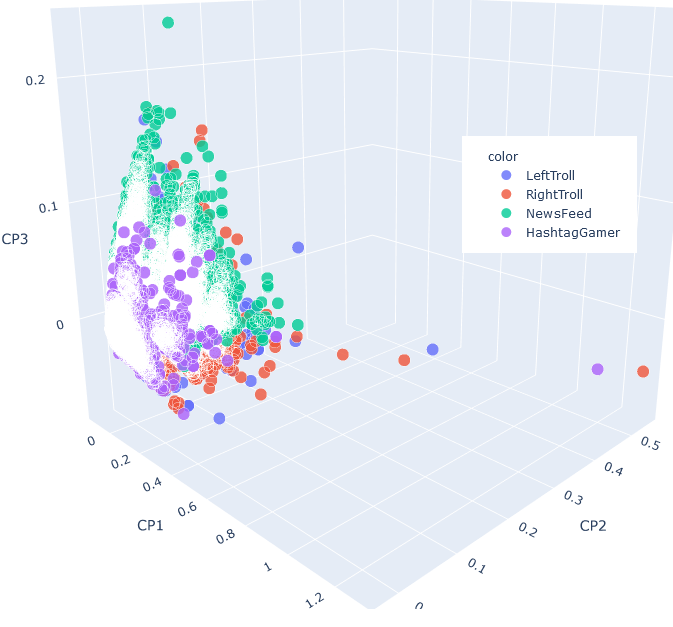
\includegraphics[width=0.45\textwidth]{Ressources/200000ACP.png}
\end{center}
\end{figure}

Les tweets sont bien regroupés selon leur catégorie quand on s'éloigne de l'origine, mais pour les scores faibles, proches de l'origine, c'est près de la moitié des tweets qui sont regroupés sans que l'on puisse distinguer des groupes par catégories.

Nous avons ensuite mis en œuvre l'algorithme KNN pour K allant de 1 à 100, avec différentes divisions aléatoires des données, pour trouver le paramètre optimal du nombre de voisins. La précision du modèle en fonction de K est représentée sur la \textsc{figure} \ref{fig:KNNACP2}.

\begin{figure}[h]
\begin{center}
\caption{\label{fig:KNNACP2}Précision de la méthode KNN après une ACP pour 200 000 tweets. K-optimal de 23 voisins.}
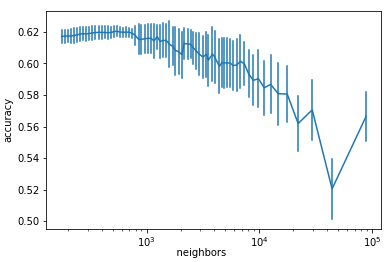
\includegraphics[width=0.45\textwidth]{Ressources/KNNacp200000.png}
\end{center}
\end{figure}

Le résultat est plutôt bon (62\% de précision), mais lorsque l'on augmente le nombre de données le classifieur perd en qualité: on tombe à 56\% de précision pour un K optimal de 90 voisins. On peut cependant poser en conjecture que le K optimal est bien plus grand en réalité, mais le temps de calcul devient trop important pour que nous le cherchions.

Pour tenter de diminuer le temps de calculs, nous avons mis en œuvre l'algorithme des \textit{K plus proches prototypes}. Cette variante de la méthode des \textit{K plus proches voisins} comporte une phase d'apprentissage constituée du calcul des prototypes qui résument les individus d'apprentissage dans chaque classe. Cependant, les performance sont restées un peu en dessous de celles des \textit{K plus proches voisins}.

Enfin, sans ACP et sur un jeu réduit des données la méthode des KNN nous a donné de bons résultats comme on pouvait s'y attendre. La \textsc{table} \ref{tab:PKPP} qui suit résume les résultats des méthodes KPP:

\begin{table}[htbp]
\begin{center}
\noindent\begin{tabular}{llll}
Tweets & ACP & K-opt & Précision au K-opt \\ 
\hline 
200 000 & 3D & 23 & 0.62 \\
1 000 000 & 3D & 90 & 0.56 \\
200 000 & non & 172 & 0.63 \\
\end{tabular}
\caption{\label{tab:PKPP} Précisions des méthodes KPP.}
\end{center} 
\end{table}

Finalement, les méthodes de K plus proches voisins sont trop gourmandes en calculs pour répondre à notre problématique. Nous en feront un meilleur usage en fin d'analyse quand nous modifieront légèrement celle-ci en nous intéressant à la classification des comptes plutôt que des tweets, ce qui réduira considérablement la taille des données d'entrée.

\subsubsection{Arbres de décision et forêts}

Les méthodes à base d'arbres binaires consistent à partitionner de manière récursive
l'espace des caractéristiques en régions homogènes au sens de notre classification.

Pour augmenter la robustesse de cette classification, on applique la technique du \textit{bagging} qui consiste à faire voter plusieurs classifieurs entraînés sur des sous-ensembles de données différents. Pour maximiser la diversité de ces classifieurs, on passe directement par la méthode des forêts aléatoire. En effet, les descripteurs utilisés pour la construction de chaque arbre sont tirés au sort (on en tire le nombre optimal, soit $\sqrt{9}=3$).

On teste les classifieurs suivants, leurs résultats sont présentés dans la \textsc{table} \ref{tab:PFA}. Comme nous l'avions proposé (\textsc{Tab.} \ref{tab:DCC}), on peut ajouter à nos variables scores le nombre de liens présents dans le tweet. Cette nouvelle dimension permet d'augmenter légèrement les performances.

\begin{enumerate}[label={[\textit{RF.\theenumi}]}]
\item 50 classifieurs, 50 nœuds terminaux, variables: 8 scores.
\item 50 classifieurs, 50 nœuds terminaux, variables: 8 scores et le nombre de liens.
\item 50 classifieurs, 100 nœuds terminaux, variables: 8 scores et le nombre de liens.
\item 100 classifieurs, 100 nœuds terminaux, variables: 8 scores et le nombre de liens.
\end{enumerate}

\begin{table}[h]
\begin{center}
\noindent\begin{tabular}{r|llll}
Méthode & Gamer & Left & News & Right \\ 
\hline 
\textit{RF.1} & 0.05 & 0.20 & 0.74 & 0.84 \\
 & \multicolumn{4}{|r}{\textit{total accuracy: 0.58}} \\
\textit{RF.2} & 0.57 & 0.14 & 0.84 & 0.76 \\
 & \multicolumn{4}{|r}{\textit{total accuracy: 0.62}} \\
\textit{RF.3} & 0.58 & 0.21 & 0.84 & 0.73 \\
 & \multicolumn{4}{|r}{\textit{total accuracy: 0.63}} \\
\textit{RF.4} & 0.57 & 0.20 & 0.84 & 0.74 \\
 & \multicolumn{4}{|r}{\textit{total accuracy: 0.63}} \\
\end{tabular}
\caption{\label{tab:PFA} Précisions des forêts aléatoires.}
\end{center} 
\end{table}

Les méthodes de forêts aléatoires donnent de bons résultats tout en n'étant pas trop gourmands en calculs. De plus, ils permettent l'ajout de descripteurs qualitatifs, sans craindre un trop grand nombre de dimensions. Cependant, la précision est encore très inégale pour les différentes classes.


\subsection{Classification des comptes}

Les parties précédentes présentait la classification des tweets pris individuellement à partir de leur contenu. Comme nous l'avons vu en fin de présentation des variables scores, cette démarche n'est pas entièrement satisfaisante [\textsc{Sec.} \ref{sec:limitescores}]. La variabilité du contenu des tweets d'une même classe -- y compris pour un même compte -- ainsi que parfois l'absence d'informations sur la classe adéquate nous empêchent de toujours identifier le comportement à associer à un tweets.

Une approche plus stable est de classifier les auteurs des tweets plutôt que les tweets eux-mêmes. Chacun des auteurs est associé à un comportement principal, c'est cette classification que nous pouvons faire plus précisément.

Deux approches ont été envisagées (la \textsc{table} \ref{tab:PMC} donne leurs précisions):
\begin{itemize}
\item travailler directement en donnant des scores aux auteurs, après la concaténation du texte de tous leurs tweets.
\item associer à l'auteur la classification majoritaire de ses tweets.
\end{itemize}

La première option donne plus d'importance aux tweets très caractéristiques d'une catégorie et à ceux avec beaucoup de contenu. Nous l'avons adoptée avec la méthode des \textit{K plus proches voisins}, sans ACP et sur touts les comptes des données [\textit{CKPP}].

La seconde donne autant de poids à chaque tweets, qu'il soit caractéristique d'une classe comportementale ou inclassable. Nous l'avons adoptée avec la méthode des forêts aléatoires [\textit{CFA}].

\begin{table}[h]
\begin{center}
\noindent\begin{tabular}{r|llll}
Méthode & Gamer & Left & News & Right \\ 
\hline 
\textit{CFA} & 0.96 & 0.08 & 0.83 & 0.72 \\
 & \multicolumn{4}{|r}{\textit{total accuracy: 0.61}} \\
\textit{CKPP} & 0.55 & 0.65 & 0.75 & 0.98 \\
 & \multicolumn{4}{|r}{\textit{total accuracy: 0.84}} \\
\end{tabular}
\caption{\label{tab:PMC} Précisions des méthodes appliqués aux comptes.}
\end{center} 
\end{table}

Le résultats sont ceux espérés pour la méthode \textit{CKPP}, qui a notamment une très bonne répartition de sa précision entre les classes (une moyenne de 0.73).

La méthode \textit{CFA}, elle, prédit très mal l'appartenance du compte à la classe \textit{Left Troll}. Ce résultat n'est pas étonnant puisque cette classe a été la plus difficile à distinguer pour toutes les méthodes, elle a donc peu de chance d'être la classe majoritaire des tweets d'un compte.

Avec les variables scores que nous avons défini la solution du regroupement des informations sémantiques de tous les tweets d'un même compte est certainement la meilleur solution.

%------------------------------------------------

\section{Conclusion}\label{sec:conclusion}

Notre objectif dans cette analyse était de parvenir à classifier automatiquement les tweets de l'IRA dans différentes catégories comportementales.

Après avoir pris en main le jeu de données, nous l'avons enrichi en créant de nouvelles variables quantitatives à partir du contenu textuel des tweets afin de pouvoir mettre à l'épreuve différents algorithmes de classification.
 
Dans un premier temps, nous avons cherché à classifier les tweets pris séparément. Nous avons obtenu des précisions globalement satisfaisantes, en particulier avec les forêts aléatoires, mais nos résultats étaient limités par le fait que les tweets sont très variables et peuvent parfois être impossibles à classifier à partir de leur contenu, et ce même pour un opérateur humain.

Nous avons donc expérimenté une seconde démarche consistant à regrouper les tweets par auteur, ce qui palliait aux limites précédemment observées. Cette fois-ci, les variables quantitatives créées étaient dans la grande majorité du temps très pertinentes, et celles-ci nous ont permis, via les méthodes déjà employées, d'obtenir des résultats de classification très satisfaisants.

À travers notre classification, nous n'avons pas apporté de nouvelle information par rapport au jeu de données initial. En effet, chacun des tweets présent dans le jeu de données a été catégorisé par Linvill et Warren. Cependant, dans le cas hypothétique où de nouveaux troll tweets associés à de nouveaux comptes troll liés avec l'IRA étaient récupérés, notre solution de classification par apprentissage supervisé à partir de mesures de caractères sémantiques associées aux comptes serait un moyen rapide et pertinent de classification automatique.




%------------------------------------------------

\begin{thebibliography}{99}

\bibitem{DLPW18}
Darren L. \textsc{Linvill} and Patrick L. \textsc{Warren} (Juin 2018). 
\newblock Troll Factories: The Internet Research Agency and State-Sponsored Agenda Building. 
\newblock {\em Disponible en ligne à \href{http://pwarren.people.clemson.edu/Linvill_Warren_TrollFactory.pdf}{cette URL}}. 

\bibitem{OR18}
Oliver \textsc{Roeder} (Jul. 2018).
\newblock Why We’re Sharing 3 Million Russian Troll Tweets.
\newblock Article publié par FiveThirtyEight, {\em disponible en ligne à \href{https://fivethirtyeight.com/features/why-were-sharing-3-million-russian-troll-tweets/}{cette URL}}.

\bibitem{ODNI17}
Office of the Director of National Intelligence (Jan. 2017).
\newblock Assessing Russian Activities and Intentions in Recent US Elections (ICA 2017-01D).
\newblock {\em Available online at \href{https://www.dni.gov/files/documents/ICA_2017_01.pdf}{this URL}}.

\bibitem{SCRM19}
Special Counsel Robert S. Mueller (March 2019).
\newblock Report On The Investigation Into Russian Interference In The 2016 Presidential Election Volume I of II.
\newblock {\em Available online at \href{https://edition.cnn.com/2019/04/18/politics/full-mueller-report-pdf/index.html}{this URL}}.
\end{thebibliography}


\bibliographystyle{plain}
\bibliography{Biblio}


\end{document}





















%
%\begin{algorithm}
%\SetKwData{Left}{left}\SetKwData{This}{this}\SetKwData{Up}{up}
%\SetKwFunction{Union}{Union}\SetKwFunction{FindCompress}{FindCompress}
%\SetKwInOut{Input}{input}\SetKwInOut{Output}{output}
%\Input{A bitmap $Im$ of size $w\times l$}
%\Output{A partition of the bitmap}
%\BlankLine
%\emph{special treatment of the first line}\;
%\For{$i\leftarrow 2$ \KwTo $l$}{
%\emph{special treatment of the first element of line $i$}\;
%\For{$j\leftarrow 2$ \KwTo $w$}{\label{forins}
%\Left$\leftarrow$ \FindCompress{$Im[i,j-1]$}\;
%\Up$\leftarrow$ \FindCompress{$Im[i-1,]$}\;
%\This$\leftarrow$ \FindCompress{$Im[i,j]$}\;
%\If(\tcp*[h]{O(\Left,\This)==1}){\Left compatible with \This}{\label{lt}
%\lIf{\Left $<$ \This}{\Union{\Left,\This}}
%\lElse{\Union{\This,\Left}}
%}
%\If(\tcp*[f]{O(\Up,\This)==1}){\Up compatible with \This}{\label{ut}
%\lIf{\Up $<$ \This}{\Union{\Up,\This}}
%\tcp{\This is put under \Up to keep tree as flat as possible}\label{cmt}
%\lElse{\Union{\This,\Up}}\tcp*[h]{\This linked to \Up}\label{lelse}
%}
%}
%\lForEach{element $e$ of the line $i$}{\FindCompress{p}}
%}
%\caption{Génération du score d'un tweet pour une classe}\label{algo_disjdecomp}
%\end{algorithm}